%
% A Real Chapter
\chapter{Background}\label{chap:background}
In this chapter, a brief background is given on legged systems, humanoid robotics at \ac{IHMC} and related works to \ac{CoM} height variation.
% Modeling of Walking
\section{Legged System Preliminaries}
In this section, commonly used expressions and background related to legged systems are briefly presented.
\subsection{Human Balancing Strategies}
As humanoid robots are a derivation of humans, human balancing strategies are briefly discussed. In \figref{fig:human}, balancing strategies are shown for a standing human. The `ankle strategy', `hip strategy' and stepping strategy are most commonly considered as a balancing strategy. However, the figure includes the `suspensory strategy' \cite{hasson1994clinical}, which is less commonly considered. With the `suspensory strategy', the human is in a slightly lower configuration with bent knees to have more control authority of the ankles.

Height variation is often not considered for a standing human. A reason for this might be that the human is often assumed to stand with straight legs. The goal of the `suspensory strategy' however, gives an interesting insight to the problem. Using height changes for balance control, the control authority of the ankles will change. Therefore, height variations for balance control could be a trade-off between the application of additional force and the gain in height. 

For dynamic cases, like walking or jumping, \ac{CoM} height variations for balance on a human can be observed in, for example, the landing after a long jump. Bending the legs and lowering the height is crucial for not falling backwards.
\begin{figure}
\centering
\includegraphics[width=0.5\textwidth]{STYLESTUFF/humanbalance.jpg}
\caption{Balancing strategies for a standing human \cite{hasson1994clinical}. (A) shows the `ankle strategy'. (B) shows the `hip strategy'. (C) shows the `suspensory strategy'. (D) shows the stepping strategy.}
\label{fig:human}
\end{figure}
% Ground Reference Points
\subsection{Ground Reference Points}\label{sec:grp}
In biped locomotion, the dynamics of the system are often simplified by considering the forces resulting from ground contact, the \ac{CoM} location and the angular moment about the \ac{CoM}. The contact forces are commonly summed up in a single \ac{GRF}, coming from a single point of application in the supporting area of the walker. Ground reference points are used to describe the dynamics of the system in a single point, using \ac{GRF} and \ac{CoM} states.

% ZMP
\subsubsection{Zero Moment Point \& Center of Pressure} 
The point on the ground where the resulting \ac{GRF} does not produce any moment in the horizontal plane at the point of application, is referred to as the \ac{ZMP} \cite{sardain2004forces}. By definition, this is the point where the part of the \ac{GRF} that does not cause angular momentum around the \ac{CoM} intersects with the ground surface. The \ac{ZMP} was initially introduced in \cite{vukobratovic1969contribution}. The \ac{ZMP} is formulated as:
\begin{equation}
    \rzmp=\cxy-\frac{\fgrxy}{\fgrz}z+\frac{\taucom}{\fgrz},
\end{equation}
where $\rzmp = [x_{zmp}, y_{zmp}]^T$ is the \ac{ZMP} location, $\fgrxy=[\fgrx,\fgry]^T$ and $\fgrz$ are the horizontal and vertical components of the \ac{GRF} respectively, $\cxy = [x,y]^T$ and $z$ are the horizontal and vertical components of the \ac{CoM} Cartesian position and $\taucom = [-\tau_y,\tau_x]^T$ is the torque about the \ac{CoM} in the horizontal plane. 

In \figref{fig:zmpvscmp} the definition of the \ac{ZMP} is visualized for two different modeling choices, using both a connection between the ankle and the \ac{CoM} as a prismatic joint. In \figref{fig:3dlipfoot}, no inertia is considered around the \ac{CoM} and the \ac{GRF} $\fgr$ coming from the \ac{ZMP} intersect with the mass $m$. The difference in position between the ankle location and the \ac{ZMP} is affected by the ankle torque $\tauankle$. In \figref{fig:3dlipfootinertia}, body inertia of the system is approximated by adding a flywheel with inertia $\inert = [I_x, I_y]^T$ to the model. The \ac{GRF}, coming from the \ac{ZMP}, can be pointed away from the \ac{CoM} by using the body torque $\taucom = [\tau_x, \tau_y]^T$ as input. 

% CoP
The \ac{CoP} coincides during walking over flat ground with the \ac{ZMP} \cite{vukobratovic2004zero}. The two points however are not equal in more complex environments. The \ac{CoP} is restricted to be located in the support polygon, while the \ac{ZMP} is restricted to be located on the ground plane  \cite{sardain2004forces}. Traditionally, the \ac{CoP} is a measured quantity from a force pressure plate under the foot. In this thesis, the \ac{CoP} location is denoted as $\rcop = [x_{cop}, y_{cop}]^T$ and considered equal to $\rzmp$, as a flat contact surface is used as reference.
%The \ac{CoP} is linked to the \ac{GRF}-moment, while the \ac{ZMP} is related to the effects of external forces on the \ac{CoM} state \cite{sardain2004forces}. 
\begin{figure}
\centering
\begin{subfigure}{0.49\textwidth}
\centering
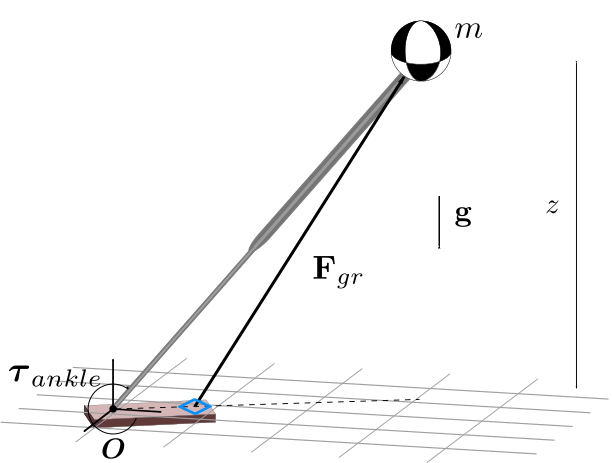
\includegraphics[width=.95\linewidth]{STYLESTUFF/3DCoPviz1.png}
\caption{}
\label{fig:3dlipfoot}
\end{subfigure}
\begin{subfigure}{0.49\textwidth}
\centering
\includegraphics[width=.95\linewidth]{STYLESTUFF/3DCMPCoPviz1.png}	
\caption{}
\label{fig:3dlipfootinertia}
\end{subfigure}
\caption{Ground reference points for different modeling choices. (a) The blue diamond points out the \ac{ZMP}/\ac{CoP} location. As no angular momentum is considered in the model,  this point is also the \ac{CMP}. (b) A flywheel with inertia is added to the model, the blue circle with cross points out the \ac{CMP} location and the blue diamond the \ac{ZMP}/\ac{CoP} location.}
\label{fig:zmpvscmp}
\end{figure}

% CMP
\subsubsection{Centroidal Moment Pivot} 
The \acf{CMP} includes, unlike the \ac{ZMP} and \ac{CoP}, angular momentum about the \ac{CoM}  \cite{popovic2005ground}. This is defined as the point where a line passing through the \ac{CoM}, parallel to the \ac{GRF} intersects with the ground surface. Unlike the \ac{CoP}, the \ac{CMP} is not constrained to lie inside the support polygon. The \ac{CMP} is defined as:
\begin{equation}
    \rcmp=\cxy-\frac{\fgrxy}{\fgrz}z,
    \label{eq:cmp}
\end{equation}
where $\rcmp =[x_{cmp}, y_{cmp}]^T$ is the \ac{CMP} location. In \figref{fig:3dlipfootinertia} the difference between the \ac{ZMP} and \ac{CMP} is graphically explained. Note that without body inertia in the model, the points coincide, as is depicted in \figref{fig:3dlipfoot}. Equivalently, if $\taucom=0$, the points coincide as well.

%leg modeling
\subsection{Inverted Pendulum-Based Models}
The line between a ground reference point and the \ac{CoM} can be modeled as an inverted pendulum. In this thesis, this line is also called the \textit{virtual leg}.

\subsubsection{Linear Inverted Pendulum Model} 
For its fast, closed-form solutions, the \ac{LIP} model \cite{kajita20013d} is widely used in walking research and especially in legged robotics. The \ac{LIP} equations of motion are:
\begin{equation}
\ddcxy=\frac{g}{l}\cxy,
\label{eq:LIPeom}
\end{equation}
where $\ddcxy$ is the horizontal \ac{CoM} acceleration. At any horizontal position, a constant leg length is considered and the motion is at a constant height $l=z_0$. In \figref{fig:3dlip} the \ac{3D} motion is visualized if the \ac{CoM} is relatively far from from the base. The pendulum base lies in the origin. Because the \ac{LIP} assumption holds, the vertical component of $\fgr$ cancels out gravity acceleration: $\fgrz=mg$.\\
\begin{figure}
\centering
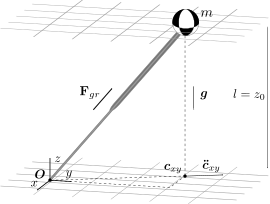
\includegraphics[width=0.5\textwidth]{STYLESTUFF/3DCoMwithoutfoot.png}
\caption{\ac{3D} motion of \ac{LIP} model.}
\label{fig:3dlip}
\end{figure}

To model body inertia of the robot, sometimes a flywheel is added to the \ac{LIP} \cite{pratt2006capture, stephens2007humanoid, koolen2012capturability}. By controlling the torque applied on the flywheel, a control authority  over the \ac{CoM} dynamics becomes available. 

% height var model
\subsubsection{Height Varying Models} 
Unlike the \ac{LIP}, height variation of the \ac{CoM} can be included in modeling of the virtual leg. Three examples of such models are:
\begin{itemize}
	\item The, not linearized, inverted pendulum model \cite{kuo2005energetic};
	\item The \ac{SLIP} model \cite{liu2015trajectory};
	\item A pendulum with prismatic joint, not constrained to maintain a constant height: the \ac{VHIP} \cite{pratt2007derivation}.
\end{itemize}
The inverted pendulum model is often used in human motion research, as in \cite{kuo2005energetic}. The advantages of a \ac{LIP}, like fast, closed-form solutions to the dynamics, are often not needed. The \ac{SLIP} model originates from hopping and running robots \cite{schwind1998spring}. Deviations from the nominal height or pendulum length are modeled as mass-spring dynamics. 

Throughout this report, special focus is given to the \ac{VHIP}. In \figref{fig:3dvhip} the \ac{VHIP} is depicted. The dynamics of the point-mass can be written in two ways. One is as a function of the \ac{GRF} in \ac{2D}:
\begin{align}
	m\ddot{x} &= \fgrtwo\frac{x}{\sqrt{x^2 + z^2}},\\
	m\ddot{z} &= \fgrtwo\frac{z}{\sqrt{x^2 + z^2}} - mg,
	\label{eq:dynamicsprattstyle}
\end{align}
where $\fgrtwo=[\fgrx, \fgrz]^T$ is the \ac{GRF} of the \ac{2D}  model. Works that use this equation are, for example, \cite{pratt2007derivation} and \cite{koolen2016balance}.

Another way of writing the dynamics of the \ac{VHIP} is as a function of the vertical acceleration $\ddot{z}$:
\begin{equation}
	\ddcxyz = \frac{g+\ddot{z}}{z}\cxyz + \vect{g},
	\label{eq:dynamicscaronstyle}
\end{equation}
where $\vect{g}=[0,0,-g]$ is the gravity force vector. The dynamical equation can be seen as a linear time-varying system. Examples of works that use the latter dynamical description for the \ac{VHIP} are \cite{hopkins2014humanoid} and \cite{caron2018balance}. Note that the two models are identical in \ac{2D}.
\begin{figure}
\centering
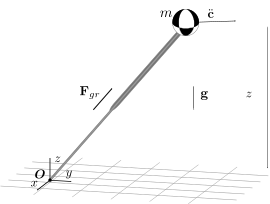
\includegraphics[width=0.5\textwidth]{STYLESTUFF/3DCoMwithoutfootVHIP.png}
\caption{\ac{3D} motion of \ac{VHIP} model.}
\label{fig:3dvhip}
\end{figure}

% Energy of Walking
\subsection{Orbital Energy \& the Capture Problem}\label{sec:ewalking}
An advantage of the \ac{LIP} is that closed-form solutions to the dynamics exists. The \ac{LIP} orbital energy is an example of such a closed-form solution. This energy can be used to determine the ability of the pendulum to converge to its unstable mode: the capture problem \cite{pratt2006capture}, \cite{koolen2012capturability}.

% LIP orbital energy
\subsubsection{Linear Inverted Pendulum Orbital Energy}\label{subsec:liporbit} 
The \ac{LIP} orbital energy is originally derived in \cite{kajita1992dynamic} and shows one of the main advantages of the use of a \ac{LIP} model.  This energy reads as follows
\begin{equation}
\Elip = \int (\ddot{x}-\frac{g}{l}x)\dot{x} dt = \frac{1}{2}\dot{x}^2-\frac{g}{2z_0}x^2,
\label{eq:Elip}
\end{equation}
where $E_{LIP}$ is the \ac{LIP} orbital energy. This orbital energy is a conserved quantity if no contact change occurs. Note that the expression resembles kinetic and potential energy: one term depends on velocity, the other on position. If $E_{LIP}>0$, the point mass will cross the horizontal position of the pendulum base with its current velocity. If $E_{LIP}<0$, the point mass will not cross the pendulum base and will have a turning point where the velocity becomes zero.

% ICP
\subsubsection{Capture Point \& Capture Region} 
More than a decade later than the first mention of the \ac{LIP} orbital energy, the \ac{CP} was presented in  \cite{pratt2006capture}. Taking $E_{LIP}=0$ and taking the square root of Equation \eqref{eq:Elip} gives
\begin{equation}
\xcplip=\sqrt{ \frac{z_0}{g}}\dot{x} 
\label{eq:cp}
\end{equation}
where $\xcplip$ is the `capture point', in this thesis referred to as the \ac{CP}. If the \ac{CoP} is held constant at the \ac{CP}, the velocity of the point-mass will be exactly driven to zero when it is above the \ac{CoP}. In \figref{fig:2dicp} a \ac{2D} visual explanation is given of this point. The \ac{CP} will be used for comparison with the \ac{VHIP} capture regions later in this report.
\begin{figure}
\centering
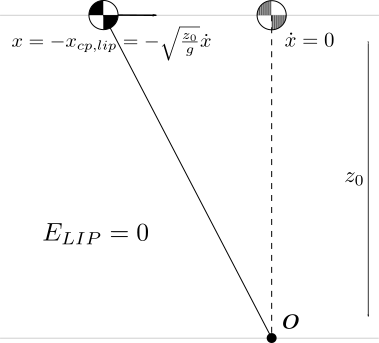
\includegraphics[width=0.4\textwidth]{STYLESTUFF/2DCP.png}
\caption{Visualization of the path to the \ac{CP}. }
\label{fig:2dicp}
\end{figure}

A capture region will traditionally appear if the \ac{LIP} plus flywheel model is used \cite{pratt2006capture, stephens2007humanoid, koolen2012capturability}. As the control authority over the flywheel can change the \ac{CoM} dynamics, a set of capture points become reachable.

\subsubsection{Instantaneous Capture Point} 
The \ac{ICP} was introduced in \cite{koolen2012capturability}, which gives a slightly different description of the \ac{CP}:
\begin{equation}
\icp=\cxy+\sqrt{\frac{z_0}{g}}\dot{\mathbf{c}}_{xy} 
\label{eq:icp}
\end{equation}
where $\icp=[\icpx, \xi_y]^T$ is the \ac{ICP}. In this way, the \ac{CP} is written in environmental coordinates and can be seen as a point where to step in the environment to come to a stop. Other similar mentions to the \ac{ICP} are the extrapolated center of mass \cite{hof2008extrapolated} and the \ac{DCM} \cite{takenaka2009real}. 
\paraskip
For planning and control, the time derivative is often taken of the \ac{ICP}: the \ac{ICP} dynamics \cite{koolen2012capturability}. This time derivative can be written as a function of the current \ac{ICP} location and a ground reference point:
\begin{equation}\label{eq:icpdyn}
\dot{\icp}=\sqrt{ \frac{g}{z_0}}(\icp-\vect{r})
\end{equation}
where $\dot{\icp}$ is the \ac{ICP} velocity and $\vect{r}$ is a ground reference point, depending on modeling choices as discussed in Section \ref{sec:grp}.

% Boundedness
%\paragraph{The boundedness condition}\label{sec:boundedness} \cite{lanari2014boundedness} includes the effects of the motion of the ground reference point in the capture problem. The solution of $x_u$, a point that also coincides with the \ac{ICP}, reads as:
%\begin{equation}
%x_u(t,r) = e^{\omega_0(t-t_0)}x_u(t_0) -\omega_0 \int_{t_0}^t e^{\omega_0(t-\tau)}r(\tau)d \tau,
%\end{equation}
%where $r(t)$ is the trajectory described by the used ground reference point, the virtual base of the pendulum. The boundedness condition reads as follows: if the the future input $r(t)$ results in convergence of the \ac
%{CoM} to the unstable mode, the following equality holds:
%\begin{equation}
%x_u(t_0) = \omega_0 \int_{t_0}^{\infty} e^{-\omega_0(\tau-t_0)}r(\tau)d \tau.
%\end{equation}
%The initial condition, which is equal to the \ac{ICP}, has to be related to $r(t)$ by this expression.

%nonlinear orbital
\subsubsection{Orbital Energy with Height Variation}\label{subsec:nonorbit} 
Allowing height variation of the \ac{CoM}, an expression for orbital energy is more difficult to derive than its linear counterpart.  Examples of attempts to include \ac{CoM} height variations in the solution to the dynamics are the time-varying \ac{DCM} \cite{hopkins2014humanoid}, the orbital energy under a virtual constraint \cite{pratt2007derivation} and the height varying boundedness condition \cite{caron2018balance}. These works are discussed in Section 
\ref{sec:relatedworksheight}, since they are highly related to the research of focus.

% Control Framework IHMC
\section{Humanoid Robotics at IHMC}\label{sec:ihmc}
To support the methods and results presented later in this thesis, this section presents a brief background on humanoid robotics at \ac{IHMC}. Most algorithms are written in Java and simulations are run in \ac{SCS}.
%robots
\subsection{Robots}
There are two humanoid robots present at the institute at the moment of writing: Boston Dynamics' Atlas \cite{koolen2016design}, \cite{kuindersma2016optimization} and NASA's Valkyrie \cite{radford2015valkyrie}. An important difference between the two robots is that Atlas is hydraulically actuated, while Valkyrie relies on electric series elastic actuators. The actuation of Atlas is in general more powerful, which allows the robot to take higher steps. Valkyrie on the other hand, has more precise torque sensing, which is important for torque control on the robot. This ties to a similarity between the robots: both robots are torque controlled. Using a control framework, the actuators of the robots can be controlled using measured and reference torque. In \figref{fig:robots}, the two robots are shown.
\begin{figure}
\centering
  \begin{subfigure}{0.49\textwidth}
  \centering
  \includegraphics[width=.6\linewidth]{STYLESTUFF/AtlasOld1.png}
   \caption{}
    \label{fig:atlas}
  \end{subfigure}
  \begin{subfigure}{0.49\textwidth}
    \centering
  \includegraphics[width=.6\linewidth]{STYLESTUFF/Valkyrie1.png}
  \caption{}
   \label{fig:valkyrie}
  \end{subfigure}
  \caption{(a) Atlas \cite{oldatlas} and (b) Valkyrie \cite{valkyrie} walking over an un-even cinder block field at \ac{IHMC}. }
  \label{fig:robots}
\end{figure}

% planning
\subsection{Planning}
In contrary to running, with walking there is a state in every cycle with two feet in contact with the ground. This is the \ac{DS} state and the state where only one leg is on the ground is the \ac{SS} state. Additionally, other states within either the \ac{DS} or \ac{SS} state are considered, like toe-off in the transition from \ac{DS} to \ac{SS}. In \ac{SS}, the leg in contact with ground is the support leg and the foot taking a step is the swing leg. The transition between those states and the duration in each state play an important role in the generation of a dynamic plan. Planning of the robots motion is conducted by separating footstep planning from dynamic planning. The dynamic plan in this case is an \ac{ICP} reference trajectory \cite{seyde2018inclusion}.
%footstepplan
\subsubsection{Footstep Planning}
Footstep planning is the generation of a sequence of footsteps for the robot to follow. A Light Detection and Ranging sensor on the head of the robot provides terrain information. One way to generate a footstep plan is to let the user define each footstep via a graphical user interface. Via relatively simple algorithmic checks on for example kinematic reachability, the user interface can show whether a footstep is feasible or not. To make this process more autonomous, recently developments have been made in the creation of a footstep planner based on a A* search algorithm. 
%icpplanning
\subsubsection{Instantaneous Capture Point Planning}\label{subsec:icpplan} 
The generation of a dynamic plan for the robot is conducted by computing an \ac{ICP} reference trajectory. This trajectory relies on the solution to the linear differential equation of the \ac{ICP} dynamics of Equation \eqref{eq:icpdyn}:
\begin{equation}\label{eq:icpsol}
	\icp(t)=e^{\omega_0t}(\icp_0- \vect{r}_0) + \vect{r}_0,
\end{equation}
where $\omega_0=\sqrt{\frac{g}{z_0}}$ is the natural frequency of the \ac{LIP} and $\icp_0$ and $\vect{r}_0$ are the initial \ac{ICP} and ground reference point location or the \textit{knot-points}. This equation assumes that the location of the ground reference point is constant. 

Under the assumption of constant ground reference point locations, the ground reference knot-points, multiple methods have been developed over the years and improvements are being made. The most traditional \ac{ICP} reference trajectory is calculated with a single \ac{ZMP} knot-point \cite{englsberger2012integration} for each footstep. For each \ac{ZMP} knot-point, an \ac{ICP} knot-point is computed by integrating the \ac{ICP} dynamics backwards in time from the last footstep to the first. Using Equation \eqref{eq:icpsol}, the local \ac{ICP} reference value can be computed at any time instance within the plan. 

The above mentioned method is extended in \cite{englsberger2014trajectory}, where multiple \ac{CMP} knotpoints per foot are considered and \ac{SS} and \ac{DS} transitions are interpolated using splines. In the most recent improvements, continous \ac{CMP} reference trajectories are used for the generation of the \ac{ICP} trajectory \cite{seyde2018inclusion}. An estimate of the angular momentum generated during the walking motion is incorporated in the generation of the \ac{CMP} reference. At the time of writing, the latter method is the one currently in use at \ac{IHMC}, and which is used for the experiments in Chapter \ref{chap:walking}.
% icp control
\subsection{Instantaneous Capture Point Control}\label{sec:icpcontrol}
Based on a \ac{CMP} and \ac{ICP} reference trajectory, the following proportional control law is used to generate a desired \ac{CMP}:
\begin{equation}
    \rcmpd=\rcmpr + \mathbf{k}_{\xi}(\icp-\icpr),
    \label{eq:rcmpd}
\end{equation}
where $\rcmpd$ is the desired \ac{CMP}, $\rcmpr$ and $\icpr$ are the reference \ac{CMP} and \ac{ICP} from the \ac{ICP} planner respectively and $\mathbf{k}_{\xi}$ is the \ac{ICP} gain. From $\rcmpd$, the desired horizontal linear momentum rate of change is computed:
\begin{equation}\label{eq:dotldxy}
    \dotldxy = \frac{\cxy-\rcmpd}{z_0}mg,
\end{equation}
where $\dotldxy$ is the desired horizontal linear momentum rate of change, which is the desired horizontal force on the \ac{CoM} of the robot. This value is sent to the whole-body \ac{QP}. Note that this value is computed based on the \ac{LIP} equations of motion. 

% momentum control
\subsection{Momentum-Based Whole-Body Control}
The desired horizontal linear momentum rate of change $\dotldxy$, the output of \ac{ICP} control, is one of the inputs for the the whole-body \ac{QP}. The whole-body \ac{QP} finds desired joint accelerations and desired \ac{GRF}, which are translated to desired joint torques by a Newton-Euler inverse dynamics algorithm.

%centroidal
\subsubsection{Centroidal Dynamics}
The constraint on the dynamics of the robot in the whole-body \ac{QP} is based on centroidal dynamics \cite{orin2013centroidal}. Centroidal dynamics describe the dynamics on and about the \ac{CoM} of the robot as a result of external forces like gravity and \ac{GRF}. To explain the \ac{CoM} dynamics for the robotic chain of the humanoid, a short introduction is given to joint to end-effector mapping. The mapping between joint velocities and end-effector motion plays a crucial role in any robotic system:
\begin{equation}\label{eq:jacobian}
\matr{T}=\begin{bmatrix}\bs{\omega} \\ \bs{\upsilon} \end{bmatrix} = \matr{J}(\qjnt)\dqjnt \in \mathbb{R}^6,
\end{equation}
where $\dqjnt$ are the joint velocities, $\matr{J}(\qjnt)$ is the Jacobian that maps joint velocities to the end-effector twist $\matr{T}$. The twist consist of the angular velocity $\bs{\omega} \in \mathbb{R}^3$ and the linear velocity $\bs{\upsilon} \in \mathbb{R}^3$. A basis for momentum-based whole-body control is the use of centroidal momentum:
\begin{equation}
\vect{h}=\begin{bmatrix}\vect{k} \\ \vect{l} \end{bmatrix} =\matr{A}(\qjnt)\dqjnt \in \mathbb{R}^6,
\end{equation}
 where $\matr{A}=\matr{I}\matr{J}$ is the inertia matrix $\matr{I}$ times the jacobian. The centroidal momentum $\vect{h}$ consists of the angular part $\vect{k} \in \mathbb{R}^3$ and the linear part $\vect{l} \in \mathbb{R}^3$. The time derivative of the centroidal momentum, the centroidal momentum rate of change, is the constraint on the dynamics of the robot in the \ac{QP} currently in use \cite{koolen2016design}:
\begin{equation}
\dot{\vect{h}}=\begin{bmatrix}\dot{\vect{k}}\\ \dot{\vect{l}} \end{bmatrix} =\matr{A}\ddot{\vect{q}} +\dot{\matr{A}}\dot{\vect{q}} = \matr{W}_g + \sum_i\matr{W}_{gr,i} + \sum_i \matr{W}_{ext,i}, 
\end{equation}
where $\matr{W}_g$ is the gravitational wrench and $\sum_i\matr{W}_{gr,i}$ the wrench exterted by the total \ac{GRF}, as a sum from the wrench at each contact point considered. The other external wrenches $\sum_i \matr{W}_{ext,i}$ can be caused for example by other contacts than ground. These are considered zero in this thesis: $\sum_i \matr{W}_{ext,i}=\vect{0}$.
%qp
\subsubsection{Whole-Body Quadratic Program} 
The whole-body \ac{QP} \cite{koolen2016design} optimizes between momentum rate objectives and motion objectives to find desired joint accelerations and desired \ac{GRF}. The optimization is formulated as follows:
\begin{equation}
\begin{array}{rlcl}
\displaystyle \min_{\bs{\ddot{q}}_d,\bs{\rho}} & \multicolumn{3}{l}{J_{\bs{\dot{h}}_d} + J_{\bs{J}} + J_{\bs{\rho}} + J_{\bs{\ddot{q}}_d} } \\%+ J_p} \\
\textrm{s.t.} & \matr{A}\ddqjntd + \dot{\matr{A}}\dqjnt = \matr{W}_g + \matr{Q}\bs{\rho}+\sum_i\matr{W}_{ext,i}\\
&\displaystyle \bs{\rho}_{min} \leq \bs{\rho}\\
&\ddot{\qjnt}_{min} \leq \ddqjntd \leq \ddot{\qjnt}_{max},
\end{array}
\end{equation}
where $\ddqjntd$ are the desired joint accelerations, $\matr{Q}\bs{\rho} = \sum_i\matr{W}_{gr,i}$ is the basis vector matrix $\matr{Q}$ times the basis vector multipliers $\bs{\rho}$. The basis vector matrix $\matr{Q}$ consists of all basis vectors of the wrench cones from each ground contact point. In \figref{fig:wrenchcone}, the wrench cone for a single ground contact point is visually explained. Currently, there are $4$ ground contact points considered for each foot of the robot.
\begin{figure}
\centering
\includegraphics[width=0.4\textwidth]{STYLESTUFF/wrenchcone.png}
\caption{Approximation of the wrench cone with basis vectors $\boldsymbol{\beta}_{ij}$ for ground contact point $i$. The linear part of the ground reaction wrench, $\vect{f}_i$ in the drawing, is a positive multiplication of the basis vectors and lies inside the wrench cone \cite{koolen2016design}. }
\label{fig:wrenchcone}
\end{figure}
The minimum $\bs{\rho}_{min}$ has to be at least zero, because of the unilateral contact constraint; the robot can only push with its feet on the ground. The total cost $J$ is composed of the following cost terms:
\begin{equation*}
\begin{array}{rlcl}
$Momentum rate objective cost:$ & J_{\dot{\vect{h}}_d}= \wght_{\dot{\vect{h}}_d}||\matr{A}\ddqjntd + \dot{\matr{A}}\dqjnt - \dot{\vect{h}}_d||^2\\
$Motion objective cost:$ & J_{\matr{J}_m} = \wght_{\matr{J}_m}||\matr{J}_m\ddqjntd-\vect{p}||^2\\
$Contact force cost:$ & J_{\bs{\rho}}=\wght_{\bs{\rho}}||\bs{\rho}||^2 \\
$Joint acceleration cost:$ & J_{\ddqjntd} = \wght_{\ddqjntd}||\ddqjntd ||^2 \\
%$Privileged configuration cost:$ & J_p = \wght_p||(\matr{I} - \matr{J}_t^{\dagger}\matr{J}_t)\ddqjntd - \ddqjntp||^2,
\end{array}
\end{equation*}
where the weighting terms $\wght$ can have a selecting function as well. For example, the centroidal momentum rate of change objective $J_{\dot{\vect{h}}_d}$ only consists of the linear part and is only affected by the desired linear momentum rate of change $\dotld$. The motion task jacobian $\matr{J}_m = [\matr{J}_1^T\quad...\quad\matr{J}_N^T]^T$ consists of all concatenated jacobians that map either joint acceleration to end-effector motion, as in Equation \eqref{eq:jacobian} or joint acceleration to joint acceleration. The motion objective vector $\vect{p} = [\vect{p}_1^T\quad...\quad\vect{p}_N^T]^T$  consists of PD-controlled desired accelerations, coming for example from trajectory tracking of the swing leg or maintaining the upper-body orientation. %The last cost term $J_p$ is determined by the privileged joint accelerations $\ddqjntp$. Here is $\matr{J}_t$ the all-task jacobian consisting of both the momentum rate objective, as well as the motion objectives. The damped Moore-Penrose pseudo-inverse  $\matr{J}_t^{\dagger} = \matr{J}_t^T(\matr{J}_t\matr{J}_t^T +\mu^2)^{-1}$ with $\mu>0$ is used in the null-space projector $(\matr{I} - \matr{J}_t^{\dagger}\matr{J}_t)$, which projects the priviliged acceleration objective in the null-space of the primary task jacobian $\matr{J}_t$. This can for example be used in singularity avoidance, where the priviliged accelerations are used to determine the configurarion of the robotic chain.  

An important note considering the research of focus is the generation of vertical \ac{CoM} motion of the robot. The desired linear momentum rate of change $\dotld$ consists, next to its horizontal component of Equation \eqref{eq:dotldxy}, of a vertical part:
\begin{equation}
\dotldz =m(k_p(z_r-z) - k_d\dot{z}), 
\label{eq:defaultheightcontrol}
\end{equation}
where $k_p, k_d$ are the PD-control gains and $z_r$ is the reference height coming from a reference trajectory. Decision variables for this trajectory are for example kinematic reachability and height changes in terrain, but maintaining the robot's balance is \textit{not} a part of those decision variables.


\subsubsection{Inverse Dynamics} 
To translate desired joint accelerations and end-effector wrenches to desired joint torques, a recursive Newton-Euler inverse dynamics algorithm is used. Desired joint torques $\bs{\tau}_d$ are calculated using the solution of whole-body \ac{QP}, $\ddqjntd$ and $\bs{\rho}$, as follows:
\begin{equation}
    \bs{\tau}_d = \matr{M}(\qjnt)\ddqjntd + \matr{C}(\qjnt,\dqjnt)\dqjnt + \matr{G}(\qjnt) + \matr{J}^T \vect{W}_{gr}.
\end{equation}
These desired joint torques are used by the torque controllers for each actuator.

A high-level overview of the control framework is shown in \figref{fig:framework}. The `high level controller' block consists for example of the \ac{ICP} controller of Section \ref{sec:icpcontrol} and the height control law of Equation \eqref{eq:defaultheightcontrol}.
\begin{figure}[h]
\centering
\includegraphics[width=0.8\textwidth]{STYLESTUFF/controlframework.png}
\caption{High-level overview of the control framework \cite{koolen2016design}. }
\label{fig:framework}
\end{figure}

% CoM Height Variation
\section{Related Work}\label{sec:relatedworksheight}
In this short literature survey, the scope is not limited to only the use of vertical \ac{CoM} motion in balance control. Other goals of improvement, like improving dynamic planning for motions over rough-terrain or for more human-like motions, are discussed as well. The methods used in these works can be closely related to \ac{MPC} and can be insightful for the problem considered in this thesis.

Traditionally, vertical \ac{CoM} motion is generated through PD control as in Equation \eqref{eq:defaultheightcontrol} \cite{kajita2003resolved, koolen2016design}. A dynamic reference plan exists, often based on the LIP model, and height variations are considered as disturbances on the model considered in the dynamical plan. Reasons to use height variations here include the guarantee of kinematic feasibility: height variation allows the robot to step up platforms, and allows the robot to take larger steps. A noteworthy, more unique, example of height variation in non-predictive control is walking with straighter legs as in \cite{griffin2018straight}. The motivation in this work is to let the robot walk more human-like, which could have more underlying benefits, such as kinematic reachability and metabolic energy consumption \cite{wang2012optimizing}.

%var height terrain
\subsection{Dynamic Planning}
Because the constant height assumption of the \ac{LIP} is constraining the dynamics of the robotic system, efforts have been made to incorporate CoM height variation in the generation of a dynamic plan. Instead of using a LIP model, a more complicated model is used. Expected height variations of the CoM can be incorporated in the dynamic planning problem, which improves the dynamic feasibility of the plan. In theory, the reference dynamics are closer to the real dynamics of the robot. Deviations from the \ac{LIP} in the \ac{CoM} reference trajectory can be incorporated in the plan. These deviations can come for example from an un-even terrain, or a human-like walking pattern.

An example of incorporating height variations in terrain in the dynamic planning problem can be found in \cite{englsberger2013three}, which is an extension of \ac{ICP} planning as in Section \ref{subsec:icpplan}. Additional reference points, similar to ground reference points as in Section \ref{sec:grp}, are designed and used in the planning method. The drawback of this method is that still a linearized model is considered and the trajectories between footsteps for the dynamical plan are constrained to be straight lines. 

In \cite{hopkins2014humanoid}, this latter aspect is improved by introducing the time-varying \ac{DCM}. The natural frequency of the \ac{LIP} was made time-varying, such that the \ac{DCM} became time-varying. However, a closed-form solution using this method was not available anymore and a dynamic plan was computed numerically.

The methods presented in \cite{brasseur2015robust} and \cite{kajita2017biped} also show the objectives of walking with straighter legs in the dynamic planning problem. The objective in the optimization in \cite{brasseur2015robust} is to let the robot walk with the straightest legs as possible at any time. In \cite{kajita2017biped}, a \ac{2D} walking pattern is generated for walking with straighter legs. The third dimension is added, under the assumption that the dynamics in the sagittal plane and the coronal plane can be decoupled. 
%balance
\subsection{Balance Control}\label{subsec:heightbalance}
Instead of coping with height variations in the dynamic planning problem, the use of \ac{CoM} height variation was recently considered as an input for online disturbance rejection. Unlike dynamic planning, in which trajectories are computed in advance, with balance control a control input needs to be computed within the control rate. When going from the \ac{LIP} to the \ac{VHIP}, the problem arises of losing the explicit solution to the dynamics. Therefore, especially in \ac{MPC}, computation times are a challenge, as reference trajectories have to be re-planned every control tick.

In this section, the following three publications that consider height variations as control input for balance are discussed. The work proposed by: Koolen, Posa \& Tedrake \cite{koolen2016balance},  Gao, Jia \& Fu \cite{gao2017increase} and  Caron \& Mallein \cite{caron2018balance}.

% 2D polynomial
\textbf{Koolen et al.} \cite{koolen2016balance} propose a \ac{2D} \ac{MPC} law, based on the \ac{VHIP} orbital energy proposed in \cite{pratt2007derivation}. This energy reads as follows:
\begin{equation}\label{eq:evhip}
    E_{VHIP}  = \frac{1}{2}\dot{x}^2\bar{f}^2(x)+gx^2f(x) - 3g\int_{x_f}^{x} f(\xi)\xi d\xi = \frac{1}{2}\dot{x}_f^2\bar{f}^2(x_f)+gx_f^2f(x_f),
\end{equation}
where $E_{VHIP}$ is the \ac{VHIP} orbital energy. The virtual constraint $z=f(x)$ is used to make a closed-form solution possible for the energy. Furthermore, $\bar{f}(x)=f(x)-f'(x)x$. Unlike its \ac{LIP} cousin, this \ac{2D} orbital energy allows for \ac{CoM} height variation. Note that filling in a constant value for the function, $f(x)=z_0$, rewrites to the \ac{LIP} orbital energy.

The function $f(x)$ is constrained to be a cubic polynomial by Koolen et al. \cite{koolen2016balance}. Using this description, four constraints are presented, which are used in a matrix to solve for the polynomial constants. There is one constraint on the final height, one constraint on the initial height, one on the initial direction and one constraint on conservation of $E_{VHIP}$. The final position of the polynomial trajectory is above the \ac{CoP} and the final velocity is zero, such that the resulting polynomial trajectory is a capture trajectory: the trajectory that results in the system to come to a stop. 

Comparable with the \ac{LIP}-based `capture regions' in \cite{pratt2006capture, koolen2012capturability} and `stable regions' in \cite{stephens2007humanoid},  Koolen et al. investigate `regions of attraction' for the \ac{MPC} law. Traditional `capture regions' consider inertia about the \ac{CoM} to control the \ac{LIP}. The \ac{VHIP} `regions of attraction' use \ac{CoM} height variation as a control input. The `regions of attraction' show an interesting insight in capture regions of the \ac{VHIP} model. By constraining the height trajectory to be a polynomial function, the \ac{MPC} law has an explicit solution. However, this comes at the cost of the trajectories, and thus also the control inputs, to be constrained to the polynomial shape. Therefore, also the regions of attraction are constrained to the polynomial shape, which can affect the regions. Furthermore, no kinematic constraints, such as a minimum and maximum height, are considered in the problem. Therefore, the control law is not implementable on a real robot without modification.

\textbf{Gao et al.} \cite{gao2017increase} present different \ac{2D} multi-step strategies to use vertical motion in balance control. An example is lowering the \ac{CoM} height in the current step, to exert more force and raise the \ac{CoM} in the next step. In this way, the pendulum can stop closer to the current position than with a \ac{LIP} trajectory. To account for the vertical \ac{CoM} motion, the natural frequency of the \ac{LIP} is adjusted with the added vertical acceleration. To make the dynamical model closed-form solvable, a constant height is considered, as the deviations from the initial height are considered to be relatively small.

% boundedness
\textbf{Caron \& Mallein} \cite{caron2018balance} propose a \ac{3D} \ac{MPC} law, based on a height varying version of the boundedness condition from \cite{lanari2014boundedness}. In \cite{lanari2014boundedness}, the boundedness condition is based on the \ac{LIP} and presents a similar expression as the \ac{ICP}, but takes a time-varying ground reference point trajectory into account.  By using a time varying natural frequency of the pendulum $\omega(t)$, Caron \& Mallein \cite{caron2018balance} combine the boundedness condition with the time-varying \ac{DCM} of \cite{hopkins2014humanoid}. By the nonlinearity of the problem, it is initially hard to solve real-time. The problem function is reformulated and written as a function of an inverse of time, rather than as a function of time. Also, the capture trajectory is divided in $10$ segments, which are considered to have a piece-wise time-invariant natural frequency. The resulting problem is solved using a nonlinear solver.

This work is expanded in \cite{caron2018capturability}. The problem is extended from `0-step' capture problems to multi-step problems. The problem formulation is rewritten and sequential quadratic programming is used to allow for fast computation times, which makes the multi-step problem also solvable real-time. Even though the work presented by Caron is the closest to application (\ac{3D} control law, kinematic and force constraints), no applied results are shown. Additionally, for the presented control laws, no comparison is made with a traditional constant height control law. Therefore, the question remains what the advantages are of the presented \ac{MPC} law compared to using a \ac{LIP}-based proportional controller for example. In Chapter \ref{chap:standing} and Chapter \ref{chap:walking} of this report, \ac{CoM} height variations in balance control are compared with constant height approaches on humanoid robots.

Comparable with the `regions of attraction' \cite{koolen2016balance}, capture regions are presented for the \ac{VHIP} model in the next chapter. Like in the approach of \cite{caron2018balance,caron2018capturability}, constraints on the kinematics and dynamics of the system are approximated with a constraint on vertical position and acceleration.